\documentclass[11pt]{article}

% Paquetes
%===================================================================================================

% Establecemos los márgenes
\usepackage[a4paper, margin=1in]{geometry}

% Separacion entre parrafos
\setlength{\parskip}{1em}

% Paquete para incluir codigo
\usepackage{listings}

% Paquete para incluir imagenes
\usepackage{graphicx}
\graphicspath{ {./images/} }

% Para fijar las imagenes en la posicion deseada
\usepackage{float}

% Para que el codigo acepte caracteres en utf8
\lstset{literate=
  {á}{{\'a}}1 {é}{{\'e}}1 {í}{{\'i}}1 {ó}{{\'o}}1 {ú}{{\'u}}1
  {Á}{{\'A}}1 {É}{{\'E}}1 {Í}{{\'I}}1 {Ó}{{\'O}}1 {Ú}{{\'U}}1
  {à}{{\`a}}1 {è}{{\`e}}1 {ì}{{\`i}}1 {ò}{{\`o}}1 {ù}{{\`u}}1
  {À}{{\`A}}1 {È}{{\'E}}1 {Ì}{{\`I}}1 {Ò}{{\`O}}1 {Ù}{{\`U}}1
  {ä}{{\"a}}1 {ë}{{\"e}}1 {ï}{{\"i}}1 {ö}{{\"o}}1 {ü}{{\"u}}1
  {Ä}{{\"A}}1 {Ë}{{\"E}}1 {Ï}{{\"I}}1 {Ö}{{\"O}}1 {Ü}{{\"U}}1
  {â}{{\^a}}1 {ê}{{\^e}}1 {î}{{\^i}}1 {ô}{{\^o}}1 {û}{{\^u}}1
  {Â}{{\^A}}1 {Ê}{{\^E}}1 {Î}{{\^I}}1 {Ô}{{\^O}}1 {Û}{{\^U}}1
  {ã}{{\~a}}1 {ẽ}{{\~e}}1 {ĩ}{{\~i}}1 {õ}{{\~o}}1 {ũ}{{\~u}}1
  {Ã}{{\~A}}1 {Ẽ}{{\~E}}1 {Ĩ}{{\~I}}1 {Õ}{{\~O}}1 {Ũ}{{\~U}}1
  {œ}{{\oe}}1 {Œ}{{\OE}}1 {æ}{{\ae}}1 {Æ}{{\AE}}1 {ß}{{\ss}}1
  {ű}{{\H{u}}}1 {Ű}{{\H{U}}}1 {ő}{{\H{o}}}1 {Ő}{{\H{O}}}1
  {ç}{{\c c}}1 {Ç}{{\c C}}1 {ø}{{\o}}1 {å}{{\r a}}1 {Å}{{\r A}}1
  {€}{{\euro}}1 {£}{{\pounds}}1 {«}{{\guillemotleft}}1
  {»}{{\guillemotright}}1 {ñ}{{\~n}}1 {Ñ}{{\~N}}1 {¿}{{?`}}1 {¡}{{!`}}1
}

% Para que no se salgan las lineas de codigo
% Para fijar una fuente que resalte
\lstset{breaklines=true, basicstyle=\ttfamily}

% Para que los metadatos que escribe latex esten en español
\usepackage[spanish]{babel}
\decimalpoint % Para que no se cambie el punto a la coma

% Para la bibliografia
% Sin esto, los enlaces de la bibliografia dan un error de compilacion
\usepackage{url}

% Para que se puedan clicar los enlaces
\usepackage{hyperref}

% Para mostrar graficas de dos imagenes, cada una con su caption, y con un caption comun
\usepackage{subcaption}

% Simbolo de los numeros reales
\usepackage{amssymb}

% Para que los codigos tengan una fuente distinta
\usepackage{courier}

\lstdefinestyle{CustomStyle}{
  language=Python,
  numbers=left,
  stepnumber=1,
  numbersep=10pt,
  tabsize=4,
  showspaces=false,
  showstringspaces=false
  basicstyle=\tiny\ttfamily,
}

% Para referenciar secciones usando el nombre de las secciones
\usepackage{nameref}

% Para enumerados dentro de enumerados
\usepackage{enumitem}

% Para mejores tablas
\usepackage{tabularx}

% Para poder tener el mismo identificador en dos tablas separadas
\usepackage{caption}

% Mostrar la página de las referencias en el indice del documento
\usepackage[nottoc,numbib]{tocbibind}

% Para mostrar las matrices
\usepackage{amsmath}

% Funciones de latex personalizadas
%===================================================================================================

% Para realizar las citas de forma corta
\newcommand{\customcite}[1]{\emph{``\ref{#1}. \nameref{#1}''}}

% Metadatos del documento
%===================================================================================================
\title{
    {Prácticas Inteligencia de Negocio}
}

\author{
    {Sergio Quijano Rey - 72103503k}\\
    {sergioquijano@correo.ugr.es} \\
    {5º Doble Grado Ingeniería Informática y Matemáticas} \\
    {Grupo de prácticas 1}
}

\date{\today}

% Separacion entre parrafos
\setlength{\parskip}{1em}

% Contenido del documento
%===================================================================================================
\begin{document}

% Portada del documento
\maketitle
\pagebreak

% Indice de contenidos
\tableofcontents

% Lista de figuras
% Uso el addtocontents para que no se muestre la seccion de indice de figuras en el indice inicial

\addtocontents{toc}{\setcounter{tocdepth}{-10}}
\listoffigures
\addtocontents{toc}{\setcounter{tocdepth}{2}}

\pagebreak

\section{Introducción}

En esta sección hablaremos de cada uno de los problemas abordados, tratando las particularidades de cada caso y algunas consideraciones en base a estas peculiaridades tratadas.

\subsection{Información general}

En todas las partes en las que necesitemos usar números aleatorios, usaremos la semilla $123456789$ para poder reproducir bajo las mismas condiciones los experimentos y para que las comparaciones entre los distintos algoritmos sean lo más justas posible. En los siguientes sub-apartados, introduciremos los distintos problemas a tratar, sus características y problemas que puedan plantear.

En todos los \emph{datasets} hemos usado la misma estructura jerárquica apoyándonos en los metanodos de \lstinline{KNIME}. Esta estructura busca una mayor limpieza en el \emph{``código''}. Dicha estructura se va a ir vislumbrando a lo largo de las secciones de estas memorias, donde incluiremos capturas de pantalla de los distintos \emph{workflows} desarrollados.

\pagebreak

\subsection{\emph{Heart Failure Prediction}} \label{intro_dataset01:seccion}

En primer lugar, la fuente original del \emph{dataset} se puede encontrar en \cite{heart_disease_dataset:online}. Aunque podemos estar trabajando con un \emph{dataset} ligeramente modificado por los profesores de la asignatura, al igual que con el resto de \emph{datasets} que estudiaremos en esta práctica.

En la propia página de la que se obtiene el dataset \cite{heart_disease_dataset:online}, se especifica que la tarea a resolver para este \emph{dataset} es \emph{``Create a model to assess the likelihood of a possible heart disease event. This can be used to help hospitals in assessing the severity of patients with cardiovascular diseases''}. Es decir, nuestra tarea es generar un modelo de clasificación para predecir, con los datos de entrada dados, si un paciente puede desarrollar algún problema de tipo cardiaco.

En el siguiente apartado, pasamos a comentar las particularidades de este \emph{dataset}, información que hemos extraído con el análisis exploratorio hecho en \lstinline{KNIME}:

\subsubsection{Análisis Exploratorio de los Datos}

Realizamos un pequeño \emph{Análisis Exploratorio Inicial} (\emph{EDA}) de los datos usando las herramientas que nos proporciona \lstinline{KNIME}.

Como ya comentábamos en \customcite{intro_dataset01:seccion}, buscamos predecir si una persona tendrá problemas de tipo cardiaco. Por tanto, la variable de salida con la que vamos a trabajar es \lstinline{HeartDisease}. Consideraremos, por su mayor relevancia, como clase positiva, a la clase $1$.

Lo primero que vemos es que tenemos $12$ variables ($11$ variables de entrada más la variable de salida) y $918$ filas (y por tanto, $918$ ejemplos).

El \emph{workflow} de mayor nivel, para este primer \emph{dataset}, se muestra en la siguiente figura:

\begin{figure}[H]
    \centering
    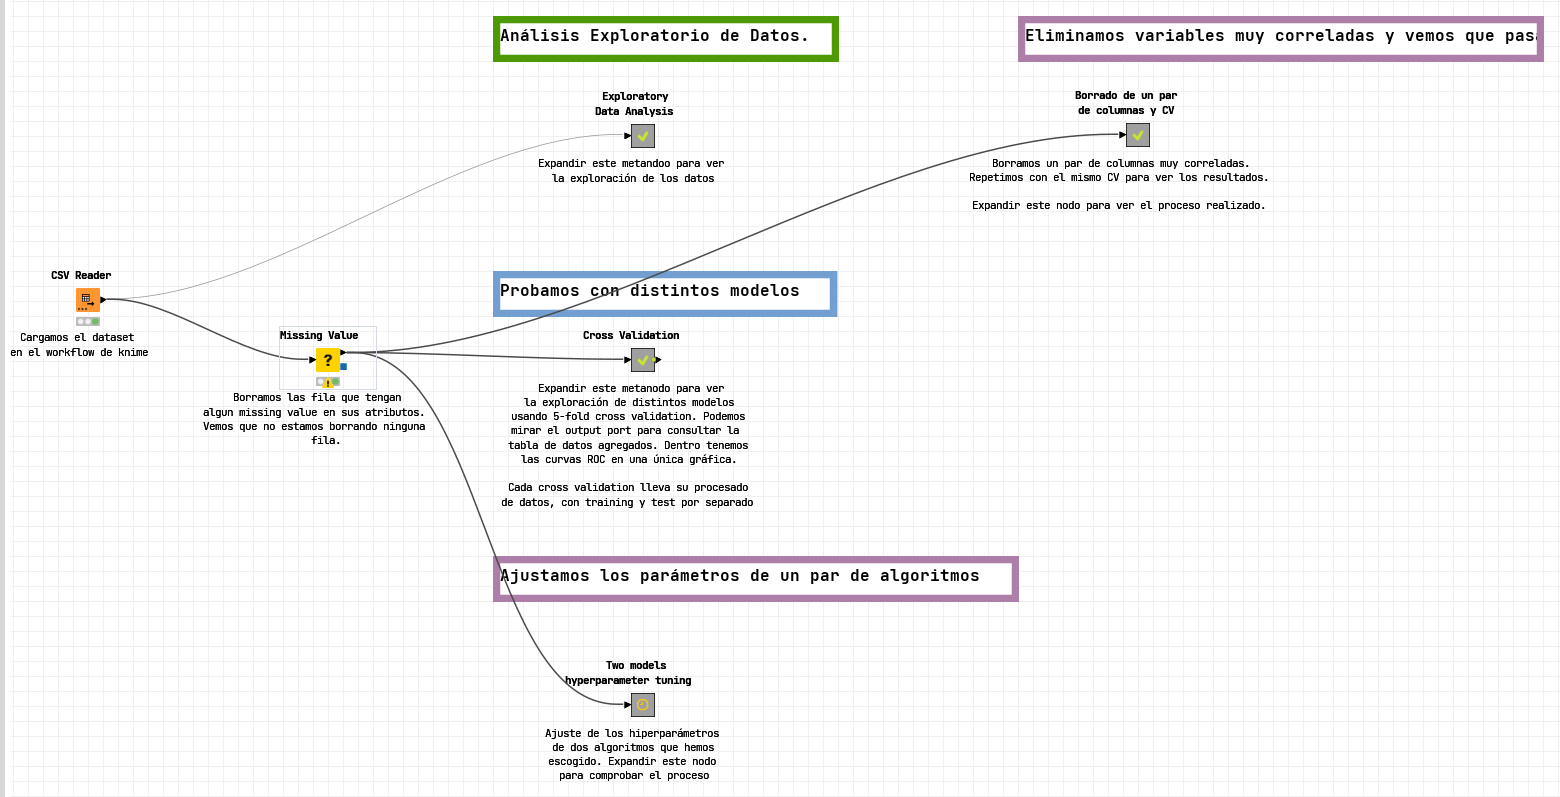
\includegraphics[width = 0.8 \textwidth]{workflow_dataset01}
    \caption{\emph{Workflow} de más alto nivel para el primer \emph{dataset}}
    \label{workflow_general:imagen}
\end{figure}

La parte que ahora nos interesa es la de Análisis Exploratorio de Datos, que mostramos en la siguiente figura:

\begin{figure}[H]
    \centering
    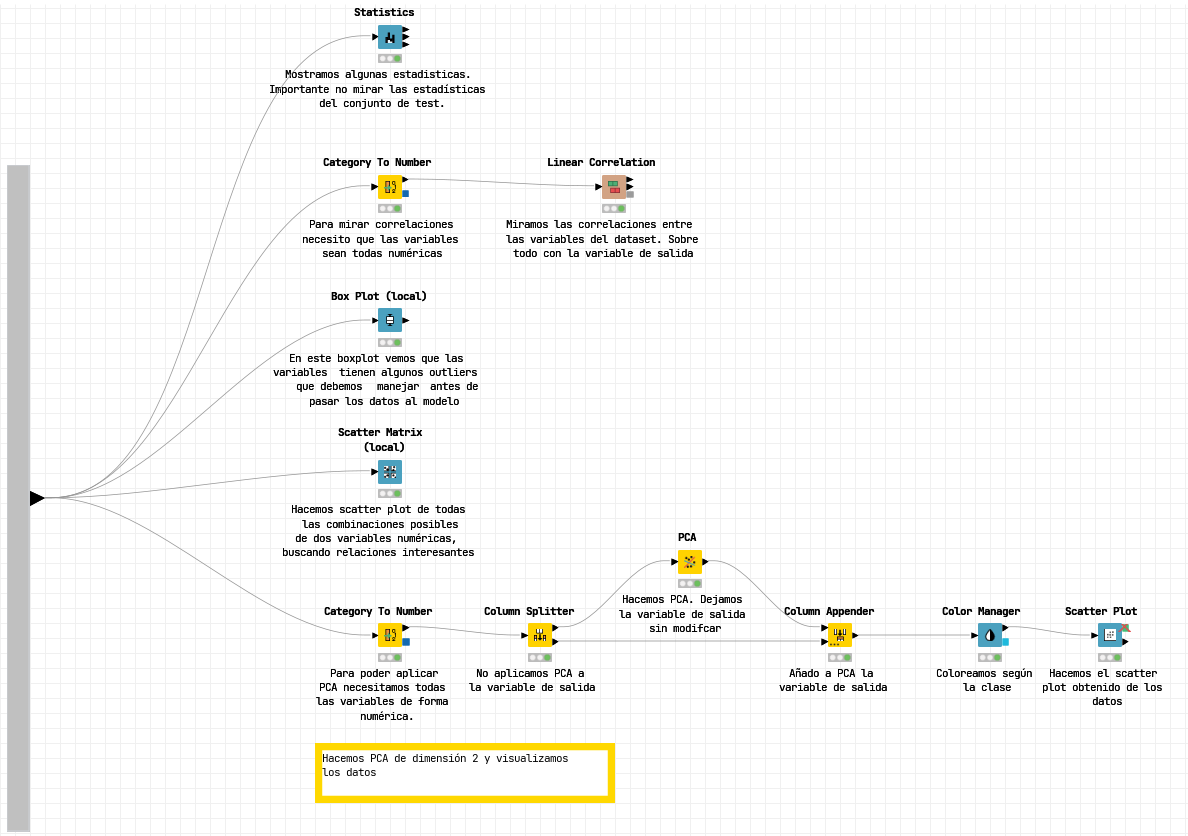
\includegraphics[width = 0.8 \textwidth]{eda_workflow_dataset01}
    \caption{\emph{Workflow} de Análisis Exploratorio de Datos para el primer \emph{dataset}}
\end{figure}

Empezamos con el nodo de estadísticas, que nos muestra que tenemos $410$ ejemplos para la clase de salida $0$ y $508$ para la clase $1$. Por tanto tenemos un ligero desbalanceo ($44.66\%$ para la clase $0$ y $55.34\%$ para la clase $1$), pero en este \emph{dataset} no vamos a tratar dicho desbalanceo. En futuros \emph{datasets} nos vamos a encontrar con clases mucho más desbalanceadas.

Dentro del anterior nodo vemos las distribuciones de las otras variables con las que trabajamos, sin llegar a conclusiones de gran relevancia, salvo razonamientos del tipo hay una característica que predomina en un valor sobre el otro valor en la población, o la población tiene una distribución de la variable normal o con cierta asimetría hacia un lado. Ejemplo de característica que predomina se muestra en la siguiente figura:

\begin{figure}[H]
    \centering
    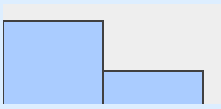
\includegraphics[width = 0.8 \textwidth]{dataset01_var_predominante}
    \caption{Distribución de la variable sexo. A izquierda, los hombres. A la derecha, las mujeres. Es claro que tenemos muchos más hombres que mujeres en nuestra población.}
    \label{variable_predominante:imagen}
\end{figure}

Esta información puede ser utilizada de forma experta en nuestros sistemas automáticos. Sin embargo, por una cuestión de tiempo, no realizamos un ajuste tan a fondo de los modelos que vamos a generar (sobre todo teniendo en cuenta que practicar esto para los cuatro \emph{datasets} es inviable. En otros \emph{datasets} realizaremos una selección de variables usando otras técnicas).

Ejemplo de una distribución con cierta asimetría se muestra a continuación:

\begin{figure}[H]
    \centering
    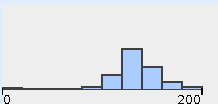
\includegraphics[width = 0.6 \textwidth]{dataset01_var_asimetrica}
    \caption{Distribución de la variable \lstinline{RestingBP}. Podemos ver claramente cómo se acumula más hacia la derecha.}
\end{figure}

De nuevo, esta información es interesante para plantear los modelos de aprendizaje automático de una forma mucho más concienzuda, pero por la extensión de la práctica en técnicas y aspectos a tener en cuenta, no entramos en detalle en este aspecto.

Lo siguiente que hacemos en el Análisis Exploratorio de Datos es mostrar la matriz de correlaciones lineales, que presentamos a continuación:

\begin{figure}[H]
    \centering
    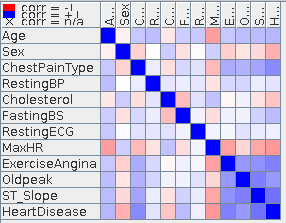
\includegraphics[width = 0.8 \textwidth]{dataset01_correlaciones}
    \caption{Matriz de correlaciones lineales. Un color azul significa correlación lineal positiva, y un color rojo significa correlación lineal negativa.}
\end{figure}

Vemos algunas variables correladas. Las más interesantes son el grupo que forman las variables \lstinline{MaxHR} \lstinline{ExerciseAngina}, \lstinline{Oldpeak}, \lstinline{ST_Slope} y la variable de salida \lstinline{HeartDisease}. Sabiendo que estas variables están muy correladas, y que una de ellas es la variable de salida, podríamos probar a construir los modelos predictivos en base a este grupo de variables. Por tanto, estamos justificando el interés de que, más adelante, probemos a eliminar ciertas filas empleando esta matriz de correlaciones, y ver cómo afecta esto al rendimiento de nuestros modelos.

Mostramos ahora los \emph{boxplots} de algunas variables, para ver que tenemos ciertos valores \emph{outliers}:

\begin{figure}[H]
    \centering
    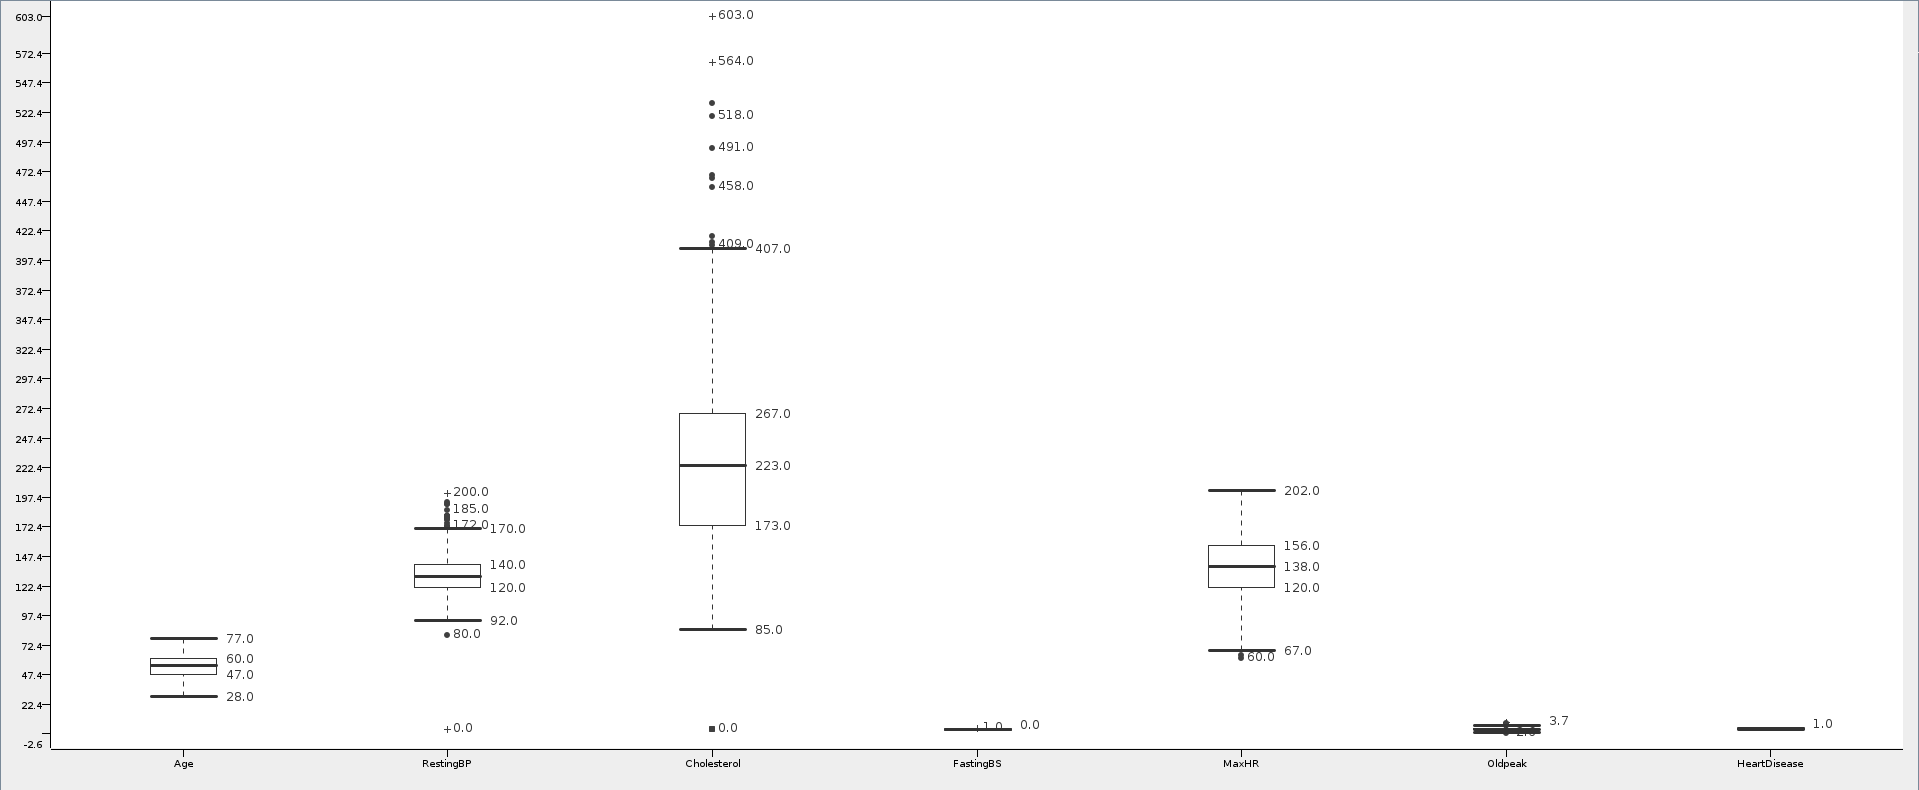
\includegraphics[width = 0.9 \textwidth]{dataset01_boxplots}
    \caption{\emph{Boxplots} de algunas de las variables con las que trabajamos. Queda claro que tenemos \emph{outliers} (sabiendo que están alejados de la media más de 3 veces la desviación típica). Por tanto, tendremos que tratar de alguna forma estos \emph{outliers}}
\end{figure}

También hacemos \emph{plots} de todas las combinaciones posibles entre dos variables, obteniendo la siguiente gráfica:

\begin{figure}[H]
    \centering
    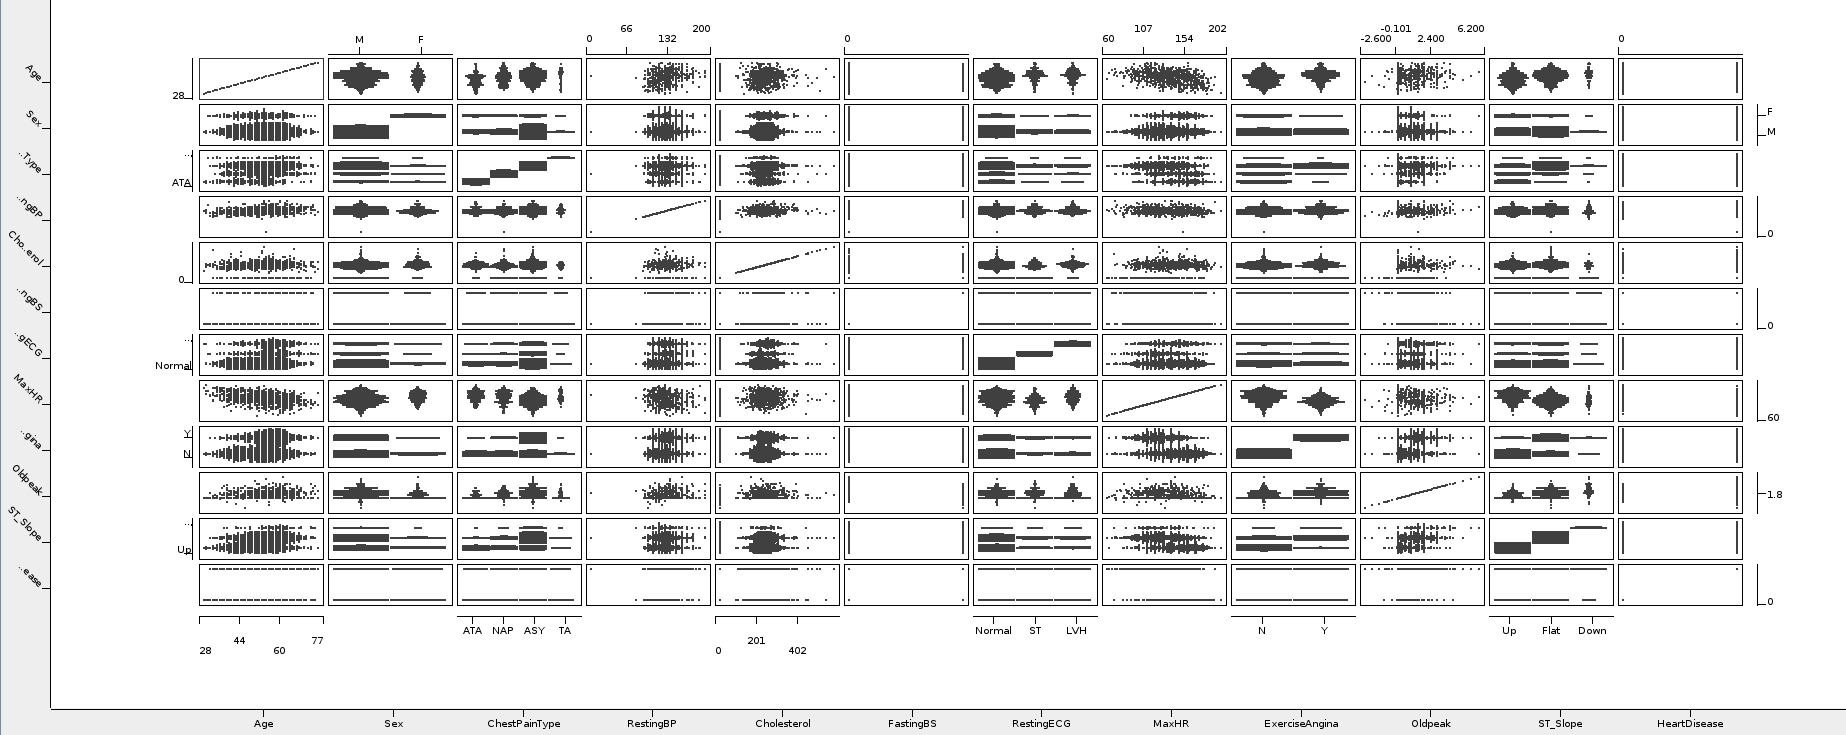
\includegraphics[width = 0.9 \textwidth]{dataset01_combinaciones}
    \caption{Gráficas de todas las posibles combinaciones de dos variables de nuestro dataset}
\end{figure}

De nuevo, como ya comentábamos para \customcite{variable_predominante:imagen}, podemos extraer de esta gráfica algunas conclusiones sobre la distribución de las variables y algunas relaciones que, por simpleza del problema y por falta de tiempo, no vamos a incluir en nuestro modelo.

En último lugar, probamos a aplicar \emph{PCA} al \emph{dataset} para obtener solo dos variables de entrada junto con la variable de salida, buscando sacar alguna información de alto nivel del problema. Esta técnica busca transformar el conjunto de datos con nuevas variables, de modo que estas variables no estén correlacionadas entre sí manteniendo el máximo posible de la varianza del conjunto de datos original. Este procedimiento se apoya en la descomposición en valores propios de la matriz de covarianzas \cite{pca:online}. Mostramos las dos variables obtenidas usando \emph{PCA}, coloreando cada punto del plano $2D$ según a la clase a la que pertenecen:

\begin{figure}[H]
    \centering
    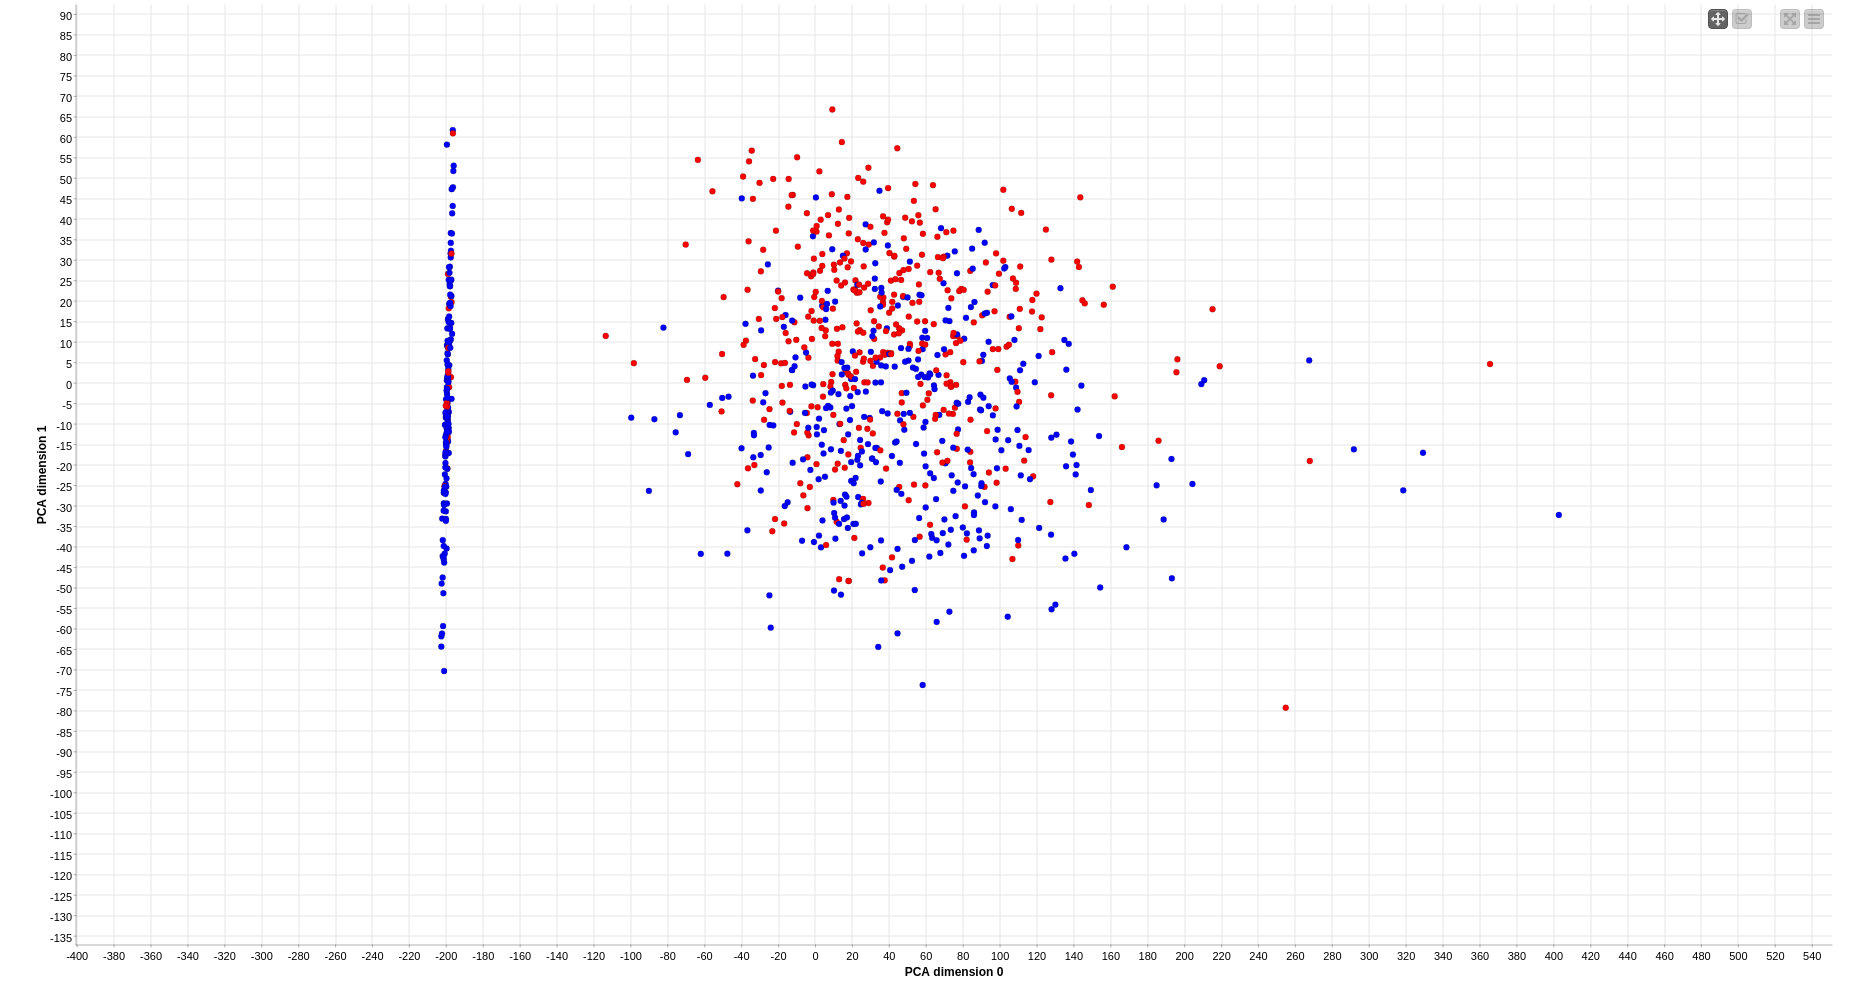
\includegraphics[width = 0.9 \textwidth]{dataset01_pca}
    \caption{Resultado de aplicar \emph{PCA} en dos dimensiones, coloreando cada punto según la clase a la que pertenecen}
\end{figure}

Los resultados obtenidos no nos invitan a usar \emph{PCA} para usarlo como base a modelos de aprendizaje automático. Sin embargo es interesante que se ha obtenido una línea a la izquierda con clara predominancia de la clase representada por el color azul, mientras que a la derecha se obtiene un \emph{clúster} ligeramente circular donde los datos de las dos clases están mezclados sin un patrón claro (quizás la clase roja tiene mayor predominancia en la parte superior). Estamos seguros de que aplicando \emph{PCA} con dimensiones mayores obtendríamos un buen \emph{performance} en los modelos de aprendizaje automático. Pero como para otros \emph{datasets} es más interesante aplicar esta técnica, lo dejamos para más adelante.

En último lugar, tratamos los \textbf{\emph{missing values}}. En el \emph{workflow} de más alto nivel, hacemos una primera aproximación al tratamiento de los \emph{missing values}. Tratamos de borrar todas las filas que contengan \emph{missing values}, pero no borramos ninguna fila. En un principio pensamos que no tenemos \emph{missing values} en este \emph{dataset}. Sin embargo, explorando la colección de datos comprobamos el siguiente hecho: la variable \lstinline{Cholesterol} contiene \emph{missing values} codificados con el valor $0$. Para tratar estos \emph{missing values}, en \emph{Cross Validation} los marcaremos como tal, y los trataremos convenientemente en cada nodo de validación (para evitar hacer \emph{data snooping}). Entraremos en detalles más adelante.

El nodo que usamos para realizar esta comprobación sobre los \emph{missing values} se muestra en el \emph{workflow} general que aparece en \customcite{workflow_general:imagen}.

\pagebreak

\section{Resultados Obtenidos}

\subsection{Consideraciones iniciales} \label{cv_consideraciones:seccion}

Para esta práctica, hemos considerado 7 modelos de aprendizaje automático distintos, que puedan ser interesantes para los cuatro problemas a los que nos vamos a enfrentar. Algunos de estos modelos pueden tener muy poco sentido para algún problema concreto. Sin embargo, elegimos los mismo 7 modelos para los 4 datasets, porque esto nos permitirá realizar una comparación entre ellos en distintos ambientes. De hecho, el que algunos modelos no tengan sentido en ciertas situaciones será una buena conclusión a extraer en el análisis posterior.

Los modelos considerados son:

\begin{enumerate}
    \item Árbol de decisión construido con \emph{AdaBoost}
    \item Red Neuronal Simple
    \item \emph{Support Vector Machine}
    \item \emph{Support Vector Machine} con normalización
    \item \emph{K-NN}
    \item \emph{Naive Bayes}
    \item \emph{Random Forest}
\end{enumerate}

Pensamos que con estos modelos tenemos una variedad suficiente para comparar en situaciones diferentes. Además, todos los los modelos tienen sentido para al menos uno de los \emph{datasets} con los que vamos a trabajar.

En este proceso, usaremos un nodo al que llamamos \emph{Custom Cross Validation}. Este nodo tiene la misma base que el nodo de \lstinline{KNIME} \emph{Cross Validation}. Sin embargo, añadimos dos nodos, uno para preprocesar el \emph{fold} de entrenamiento y otro para aplicar dicho preprocesado al \emph{test}, sin hacer \emph{data snooping}. Es decir, las operaciones se calculan y aplican con \emph{training}, y se aplican en \emph{test} \textbf{usando el cálculo realizado sobre \emph{training}}.

En \customcite{heart_failure_cross_validation:seccion} mostraremos de forma extensa los distintos \emph{workflows} que componen nuestras siete validaciones cruzadas. Sin embargo, para los siguientes \emph{datasets} no repetiremos el mismo proceso, para evitar ser demasiado repetitivos y extensos. Solo mostraremos aquellas partes en las que haya diferencias con lo mostrado en \customcite{heart_failure_cross_validation:seccion} y con los \emph{datasets} desarrollados previamente.

\pagebreak

\subsection{Heart Failure Prediction} \label{heart_failure_cross_validation:seccion}

\subsubsection{\emph{Workflows} empleados para \emph{Cross Validation}}

En primer lugar, tenemos un \emph{metanodo} para encapsular todo el trabajo con los 7 algoritmos que hemos considerado. Este \emph{metanodo} se mostraba en el \emph{workflow} más general en \customcite{workflow_general:imagen}. Dentro de este nodo para \emph{Cross Validation} tenemos la siguiente estructura:

\begin{figure}[H]
    \centering
    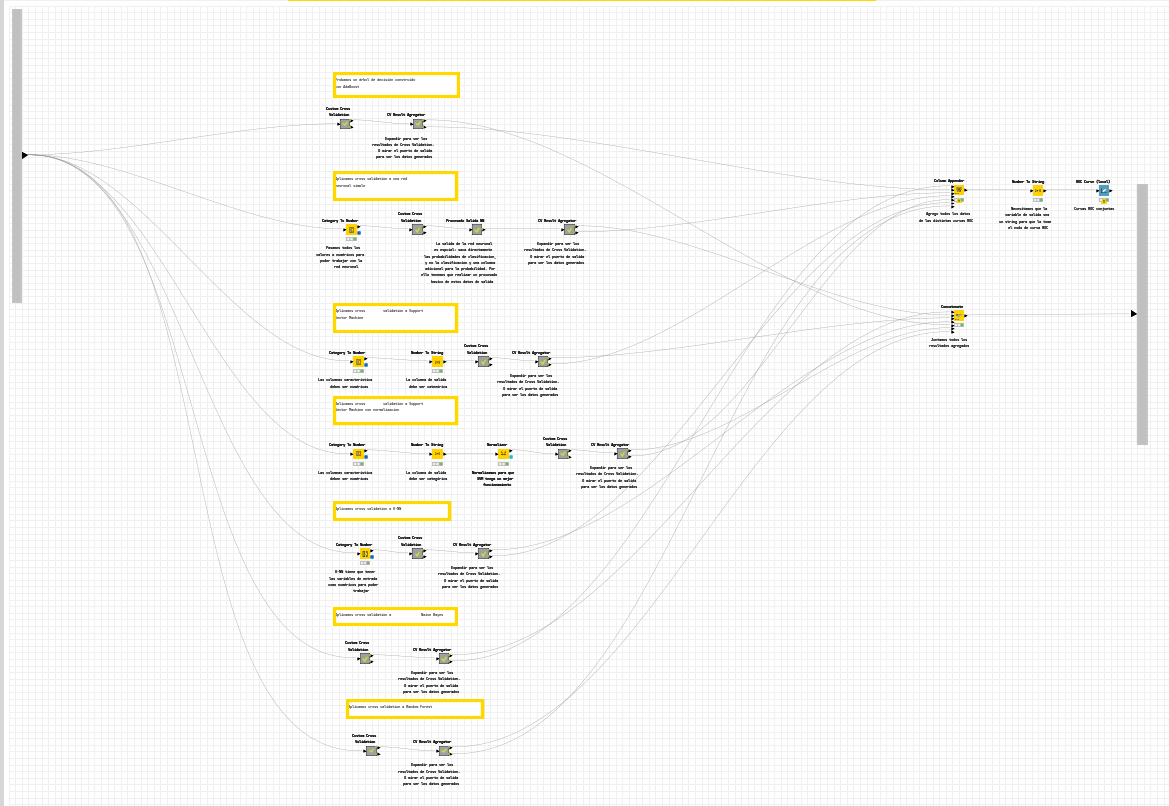
\includegraphics[width = 0.9 \textwidth]{dataset01_cross_validation_workflow}
    \caption{\emph{Workflow} en el que realizamos todos los \emph{Cross Validation} de los algoritmos considerados}
\end{figure}

Mostramos una captura con mayor \emph{zoom} para que se vea claramente la estructura generada, dejando sin mostrar alguna de las filas correspondientes a algunos de los 7 modelos estudiados:

\begin{figure}[H]
    \centering
    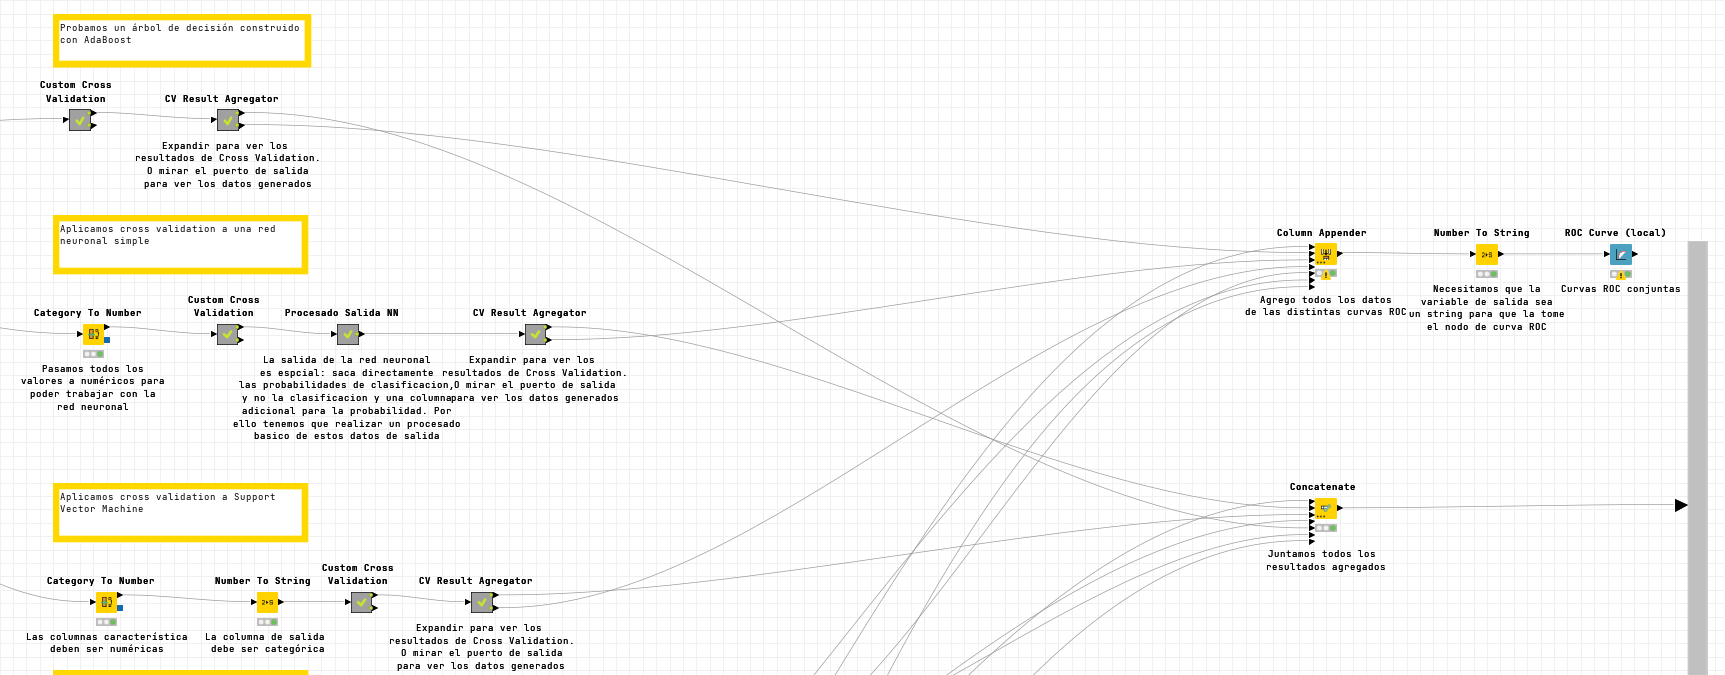
\includegraphics[width = 0.9 \textwidth]{dataset01_cross_validation_workflow_zoom}
    \caption{\emph{Workflow} en el que realizamos todos los \emph{Cross Validation} de los algoritmos considerados, con algo de \emph{zoom} para que se aprecie mejor la estructura desarrollada}
    \label{cross_val_zoom:image}
\end{figure}

Mostramos el contenido del nodo \emph{Custom Cross Validation} para \emph{AdaBoost}. Este nodo \emph{Custom Cross Validation} tiene ciertas diferencias como ya hemos mencionado en \customcite{cv_consideraciones:seccion}:

\begin{figure}[H]
    \centering
    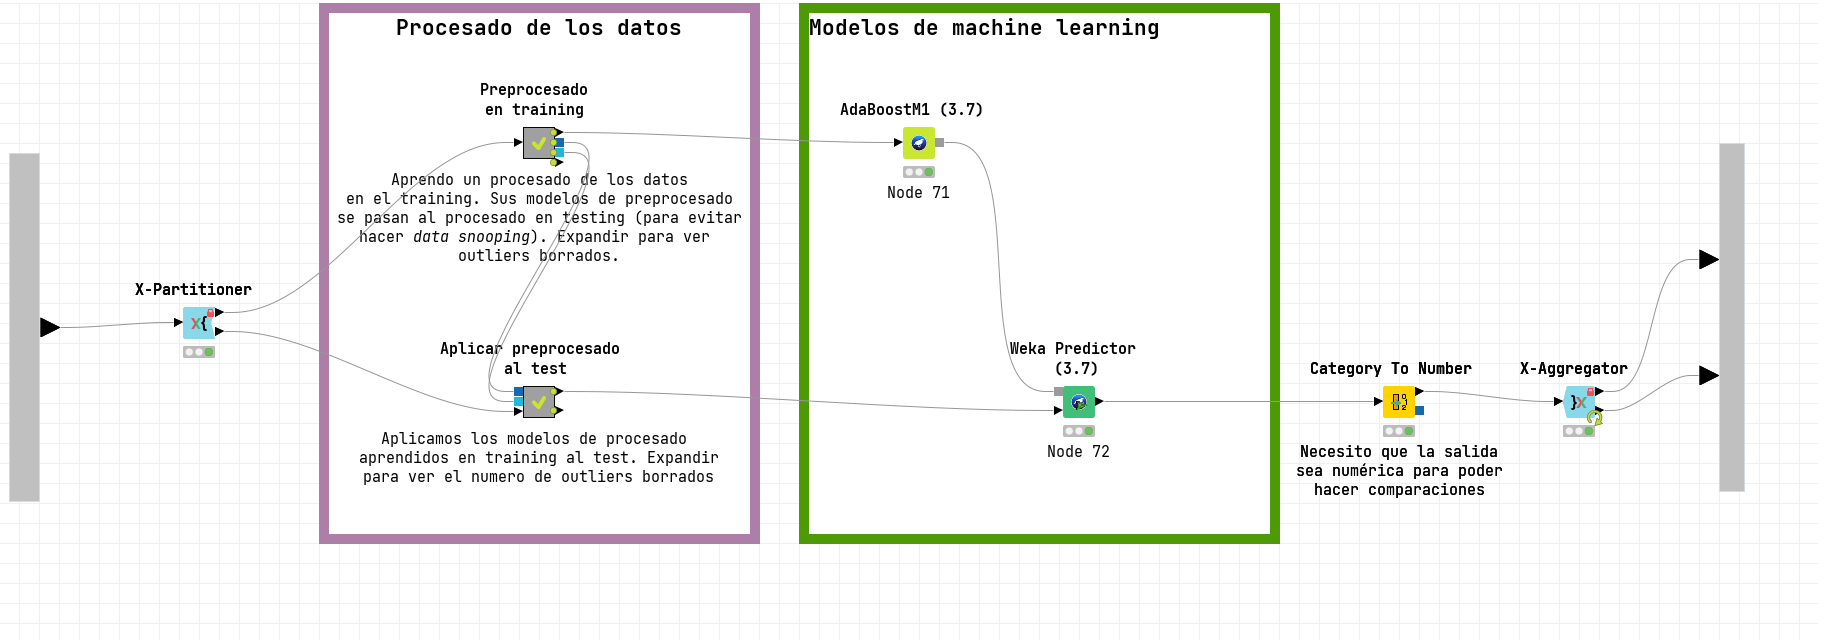
\includegraphics[width = 0.9 \textwidth]{dataset01_cv_adaboost}
    \caption{Nodo de \emph{Cross Validation} para \emph{AdaBoost}}
\end{figure}

Mostramos ahora el nodo para preprocesamiento en \emph{training}:

\begin{figure}[H]
    \centering
    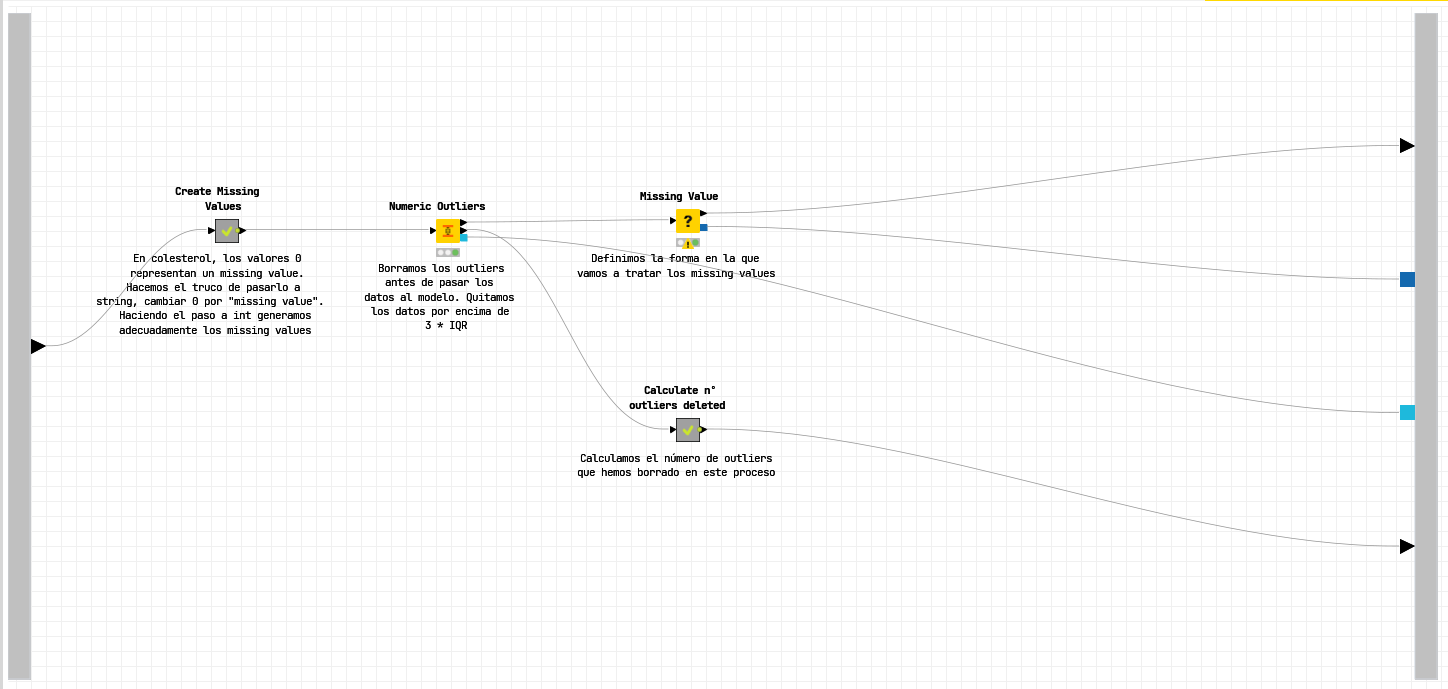
\includegraphics[width = 0.9 \textwidth]{dataset01_cv_pretraining}
    \caption{Preprocesamiento de los datos del \emph{fold} de \emph{training}}
\end{figure}

En esta figura se muestran dos partes fundamentales del procesamiento en este \emph{dataset}. La primera es que, como ya comentábamos, tenemos \emph{missing values} en la columna \lstinline{Cholesterol} marcados con el valor 0. \lstinline{KNIME} no detecta esto como \emph{missing values}, así que empleamos el nodo \emph{Create Missing Values} para marcarlos como tal.

En segundo lugar, tratamos los \emph{outliers} para intentar reducir algo el ruido. Para ello, borramos aquellos valores que distan de la media más de tres veces la desviación típica (fundamentándonos en las propiedades de una distribución normal, en la que la mayoría de los datos están en el intervalo $[\mu - \sigma, \mu + \sigma]$ \cite{intervalos_normal:online}).

Mostramos el nodo \emph{Create Missing Values} para dejar claro el proceso que hemos descrito previamente:

\begin{figure}[H]
    \centering
    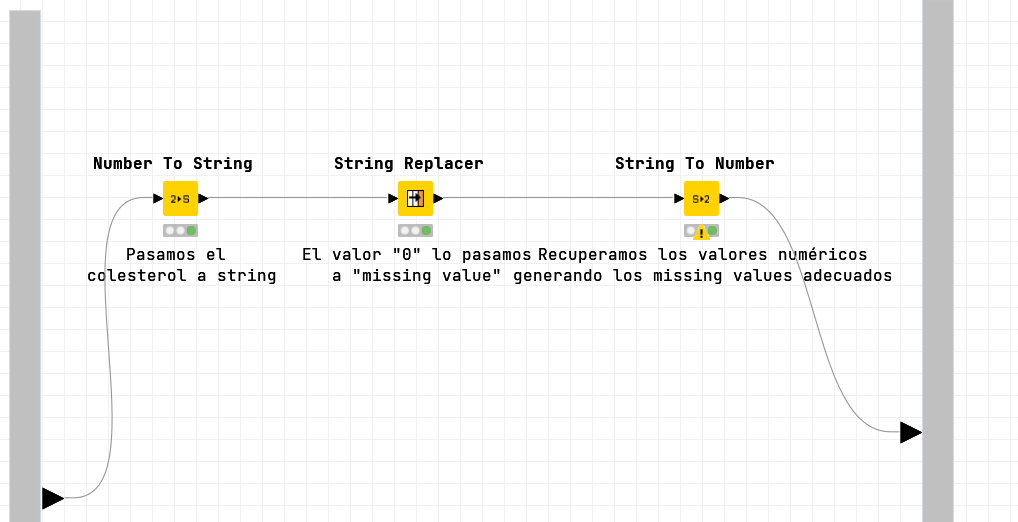
\includegraphics[width = 0.9 \textwidth]{dataset01_cv_createmissingvalues}
    \caption{Nodo que usamos para crear los \emph{Missing Values} que \lstinline{KNIME} no detecta}
    \label{pretest:imagen}
\end{figure}

Mostramos ahora el nodo para preprocesamiento en \emph{test}:

\begin{figure}[H]
    \centering
    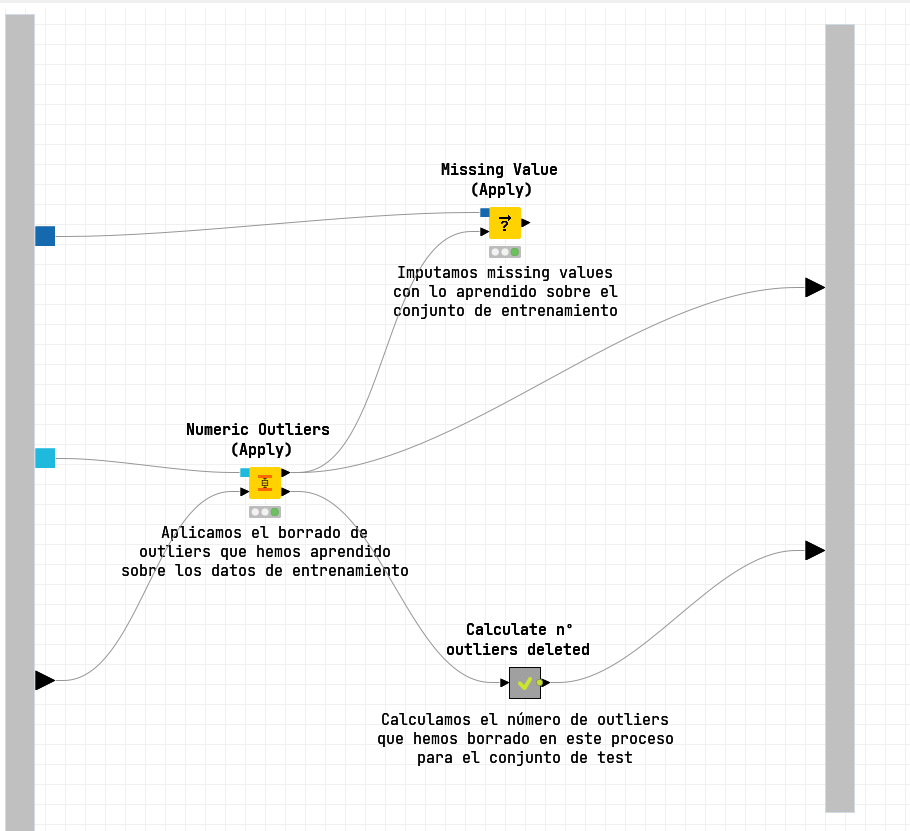
\includegraphics[width = 0.9 \textwidth]{dataset01_cv_pretest}
    \caption{Preprocesamiento de los datos del \emph{fold} de \emph{test}}
    \label{pretest:imagen}
\end{figure}

En \customcite{pretest:imagen} queda claro lo que ya comentábamos, preprocesamos usando los parámetros de procesamiento calculados sobre el \emph{fold} de \emph{training}. Esto es fundamental para \textbf{evitar hacer \emph{data snooping}}.

Además, de ahora en adelante, salvo que se diga lo contrario, estos dos nodos de preprocesamiento serán exactamente los mismos en todos los nodos de \emph{Custom Cross Validation}, en todos los \emph{dataset}, salvo que se indique lo contrario.

Como se muestra en \customcite{cross_val_zoom:image}, estamos pasando la salida de \emph{Custom Cross Validation} a un nodo de procesamiento, que mostramos a continuación:

\begin{figure}[H]
    \centering
    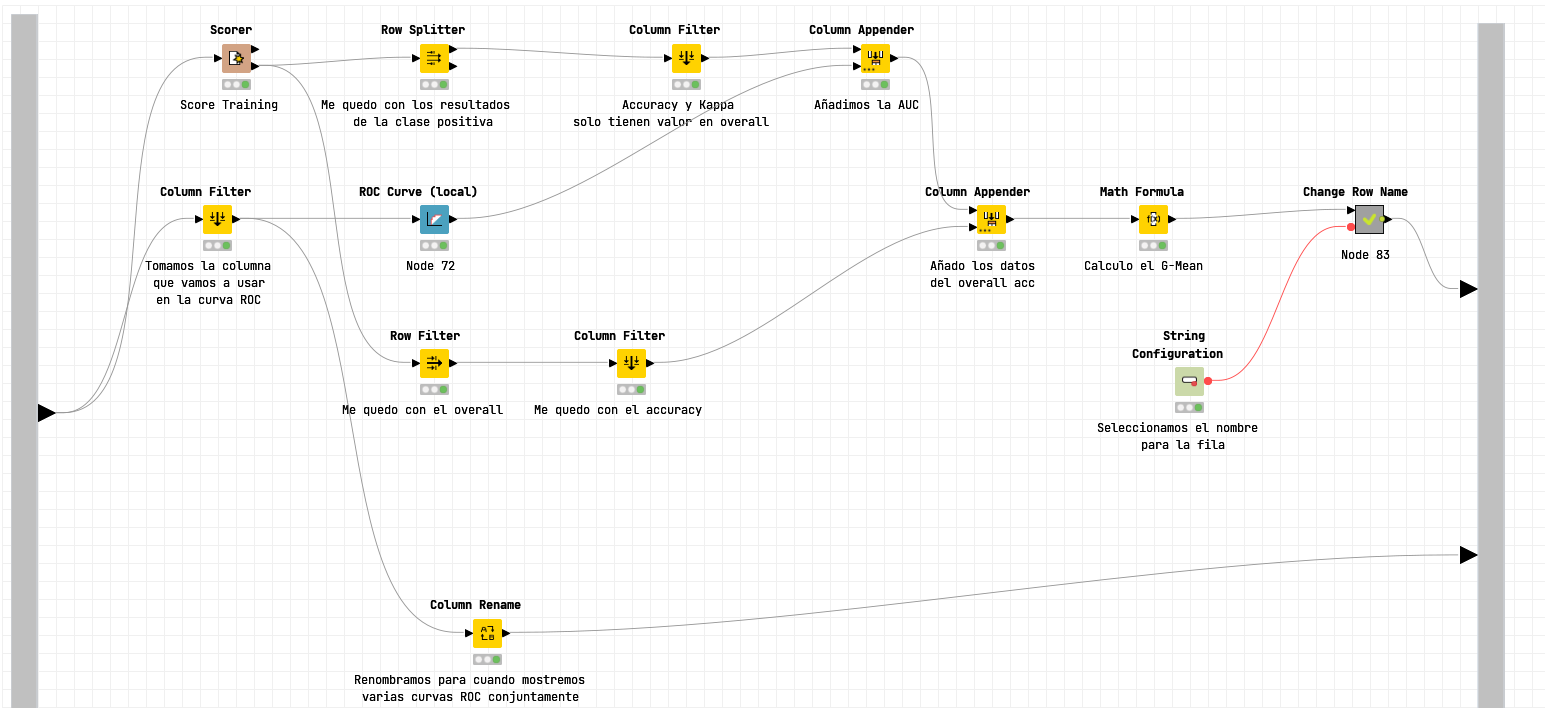
\includegraphics[width = 0.9 \textwidth]{dataset01_cv_process_node}
    \caption{Nodo de procesamiento de la salida de \emph{Custom Cross Validation}}
\end{figure}

En este nodo, tomamos la salida del \emph{scorer} y la procesamos, tomando las métricas para la clase positiva y añadiendo el área debajo de la curva \emph{ROC}. Además, calculamos la fórmula de la métrica \emph{G-Mean}. También devolvemos las probabilidades en bruto para poder calcular las curvas \emph{ROC} globales.

Se muestra también que estamos usando una \lstinline{flow variable} para establecer el nombre del modelo cuyos resultados estamos procesando. Esto es útil para que en las tablas globales, cada fila esté etiquetada por el nombre del modelo que estamos tratando (esto es lo que consigue el nodo \emph{Change Row Name}).

De nuevo, salvo que se diga lo contrario, todos los nodos de este tipo son idénticos.

Mostramos ahora el \emph{workflow} para redes neuronales simples. Realizamos un preprocesado general básico antes de usar nuestro nodo \emph{Custom Cross Validation} que mostramos en la siguiente figura:

\begin{figure}[H]
    \centering
    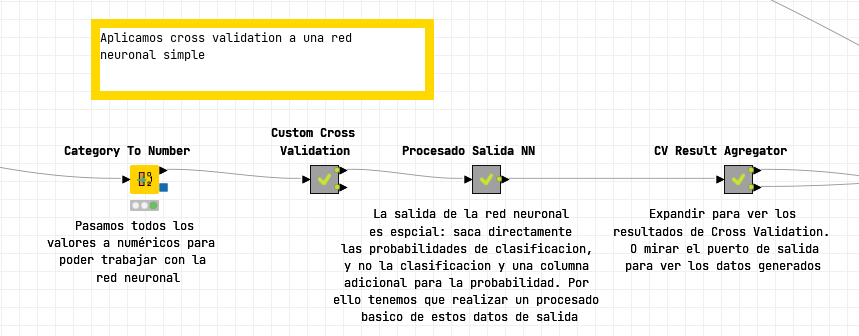
\includegraphics[width = 0.9 \textwidth]{dataset01_cv_pregeneral_nn}
    \caption{Preprocesado general previo a probar Redes Neuronales simples}
\end{figure}

Con esto queda claro que lo único que estamos realizando es pasar todas las variables categóricas a numéricas, pues esto es un requerimiento de las redes neuronales para que puedan funcionar. Mostramos el nodo de \emph{Custom Cross Validation} para este caso:

\begin{figure}[H]
    \centering
    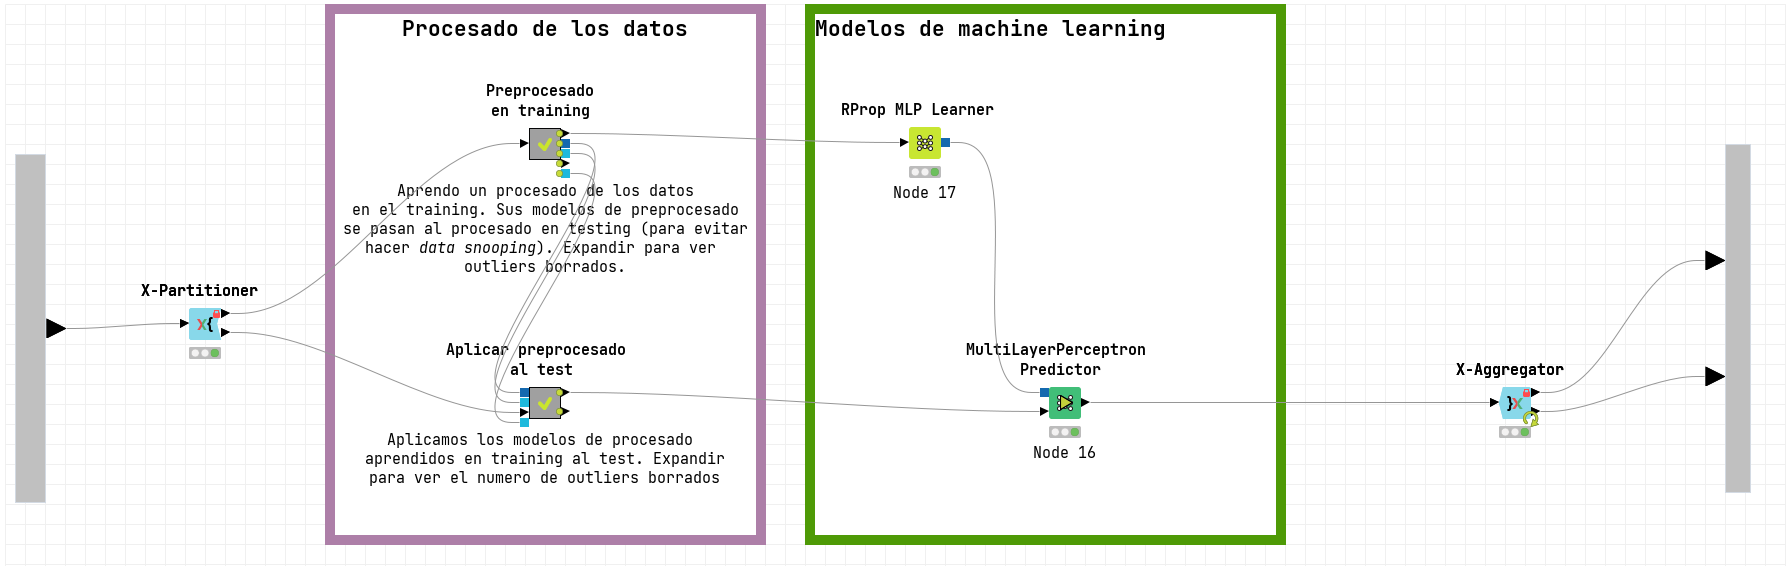
\includegraphics[width = 0.9 \textwidth]{dataset01_cv_nn}
    \caption{Nodo de \emph{Cross Validation} para \emph{Neural Net}}
\end{figure}

En este caso no estamos normalizando las variables, lo cual puede generar resultados no óptimos (pues las redes neuronales se benefician mucho de que las variables de entrada estén normalizadas. De hecho en \emph{deep learning} se usa \emph{batch normalization} para normalizar las salidas entre capas ocultas). Por simpleza del modelo no hacemos esta normalización para el \emph{dataset}, pero en siguientes \emph{datasets} sí que haremos la normalización.

La salida de las redes neuronales suponen un caso concreto que tratar. La red neuronal no nos da la clasificación directamente, sino un valor $x \in [0, 1]$. Tenemos que tratar la salida a mano. Para ello duplicamos la salida de este valor $x$ que representa la probabilidad de clasificación que usaremos para las curvas \emph{ROC}. En una de las dos ramas, colapsamos ese valor al conjunto $\{0, 1 \}$ redondeando, y consideramos eso la salida de clasificación. Mostramos ese proceso, que se hace en el nodo de \emph{Procesado Salida NN}, en la siguiente figura:

\begin{figure}[H]
    \centering
    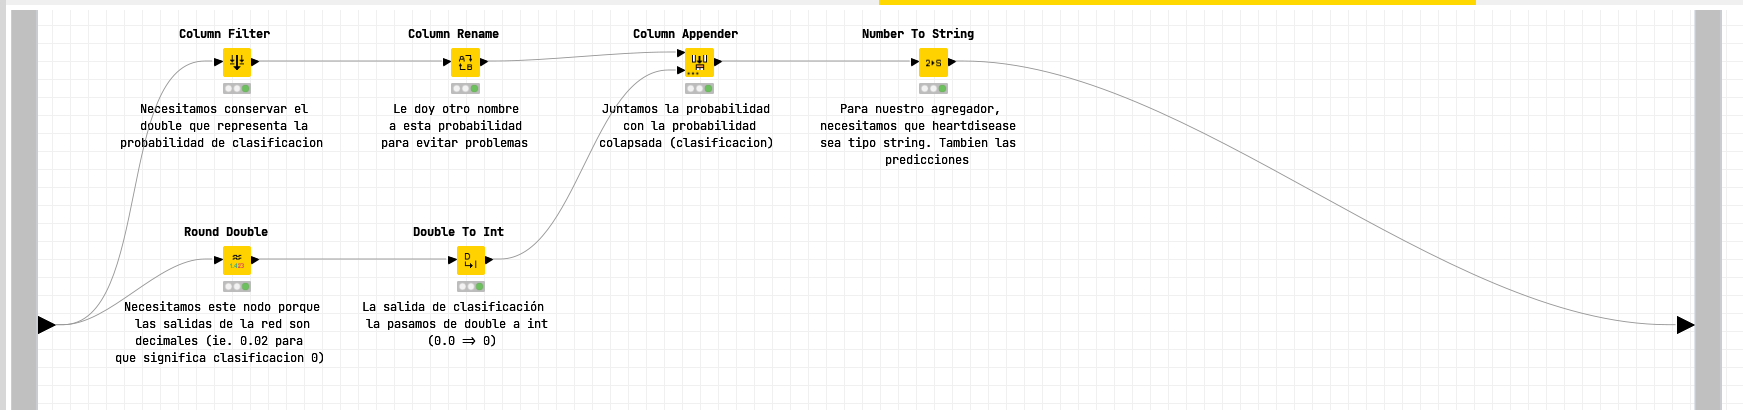
\includegraphics[width = 0.9 \textwidth]{dataset01_cv_procesado_salida}
    \caption{Procesado de la salida de \emph{Neural Net}}
\end{figure}

Con esto, usamos el nodo que procesa la salida de \emph{Cross Validation} que ya hemos mostrado previamente, y que no volvemos a mostrar para evitar ser repetitivos.

Mostramos ahora el preprocesado general para \emph{Support Vector Machine}. Consiste en pasar a variables numéricas todas las variables menos la de salida, que debe ser de tipo categórica:

\begin{figure}[H]
    \centering
    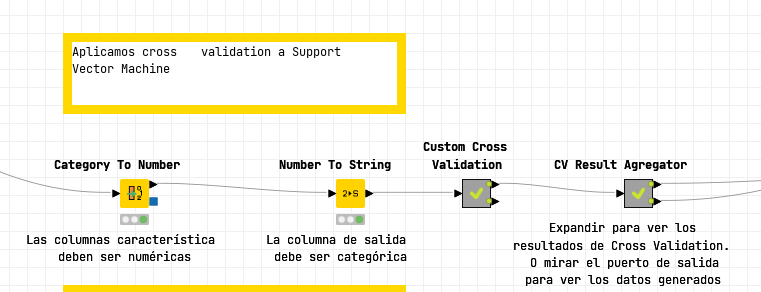
\includegraphics[width = 0.9 \textwidth]{dataset01_cv_pregeneral_svm}
    \caption{Preprocesado general previo a probar \emph{Support Vector Machine}}
\end{figure}

Mostramos ahora el nodo \emph{Custom Cross Validation} para este modelo:

\begin{figure}[H]
    \centering
    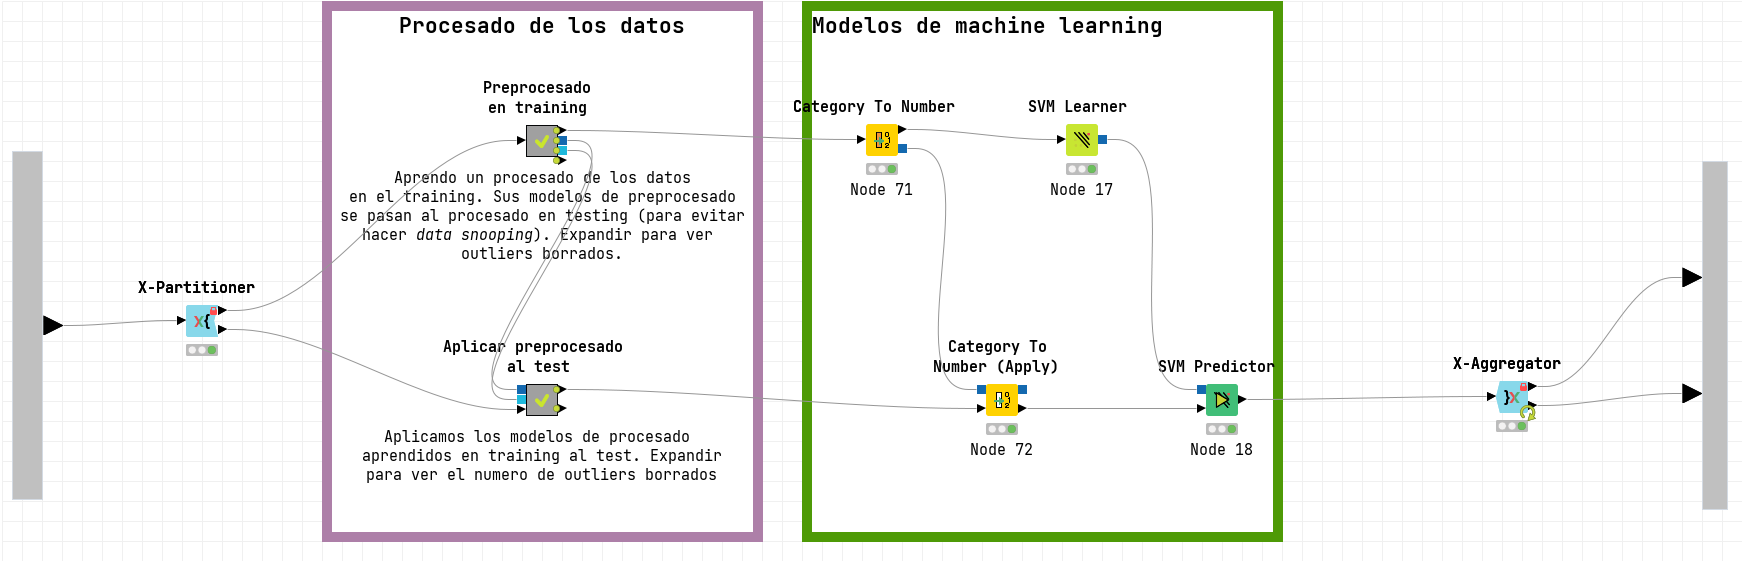
\includegraphics[width = 0.9 \textwidth]{dataset01_cv_svm}
    \caption{Nodo de \emph{Cross Validation} para \emph{Support Vector Machine}}
\end{figure}

En este caso, nos aseguramos de nuevo que estamos usando variables numéricas para las variables de entrada. En este \emph{dataset}, usamos los nodos de \lstinline{KNIME} para \emph{SVM}. En otros \emph{datasets} donde la eficiencia sea clave, pasaremos a usar los nodos de \emph{Weka} que aparentemente funcionan de forma más rápida.

En el caso de \emph{Supoort Vector Machine} con normalización, lo único que cambiamos es el preprocesado general que aplicamos antes de \emph{Custom Cross Validation}. Mostramos esto a continuación:

\begin{figure}[H]
    \centering
    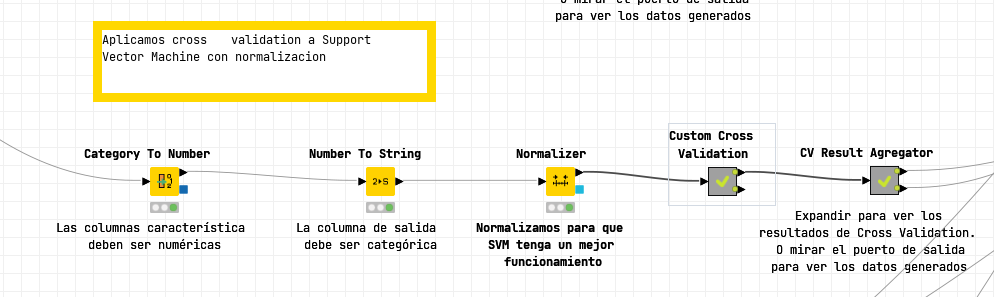
\includegraphics[width = 0.9 \textwidth]{dataset01_cv_pregeneral_svm_norm}
    \caption{Preprocesado general previo a probar \emph{Support Vector Machine} con normalización. Esto es lo único que cambia respecto al modelo anterior: \emph{SVM} sin normalización}
\end{figure}

Mostramos ahora el preprocesado general para \emph{K-NN}. \emph{K-NN} tiene que trabajar con todas las variables de entrada en formato numérico, y esto es lo que hacemos:

\begin{figure}[H]
    \centering
    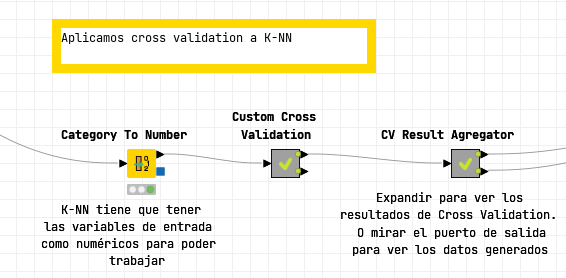
\includegraphics[width = 0.9 \textwidth]{dataset01_cv_pregeneral_knn}
    \caption{Preprocesado general previo a probar \emph{K-NN}}
\end{figure}

Dentro del nodo de \emph{Custom Cross Validation} lo que hacemos es, de nuevo asegurar que tenemos las variables en el formato correcto, y formatear la salida de \emph{K-NN} para que el nodo \emph{X-Aggregator} pueda funcionar correctamente. Mostramos esto a continuación:

\begin{figure}[H]
    \centering
    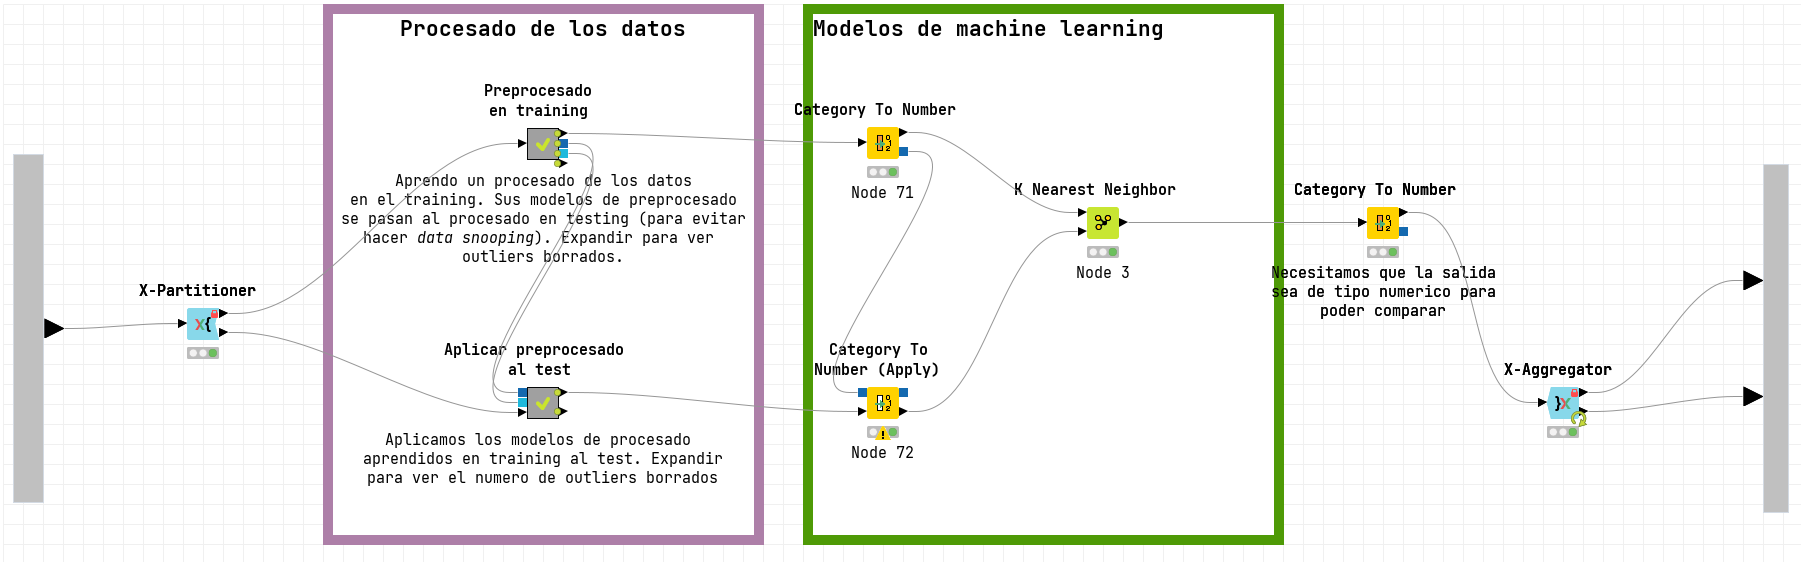
\includegraphics[width = 0.9 \textwidth]{dataset01_cv_knn}
    \caption{Nodo de \emph{Cross Validation} para \emph{K-NN}}
\end{figure}

Mostramos ahora el preprocesado general para \emph{Naive Bayes}. En este caso, no estamos realizando ningún preprocesado general:

\begin{figure}[H]
    \centering
    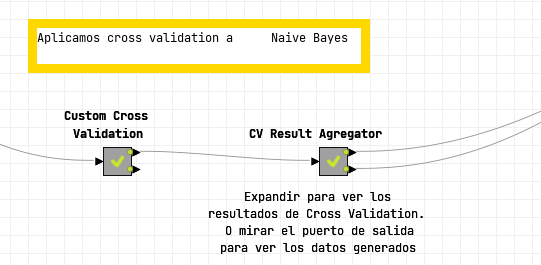
\includegraphics[width = 0.9 \textwidth]{dataset01_cv_pregeneral_naivebayes}
    \caption{Preprocesado general previo a probar \emph{Naive Bayes}. En este caso no estamos realizando ningún tipo de preprocesado previo a \emph{Custom Cross Validation}}
\end{figure}

Mostramos lo que hacemos dentro del nodo \emph{Custom Cross Validation}. No realizamos ningún preprocesado adicional además de los que ya hemos comentado previamente. La salida la pasamos a valores numéricos, para que el nodo \lstinline{X-Aggregator} pueda trabajar correctamente:

\begin{figure}[H]
    \centering
    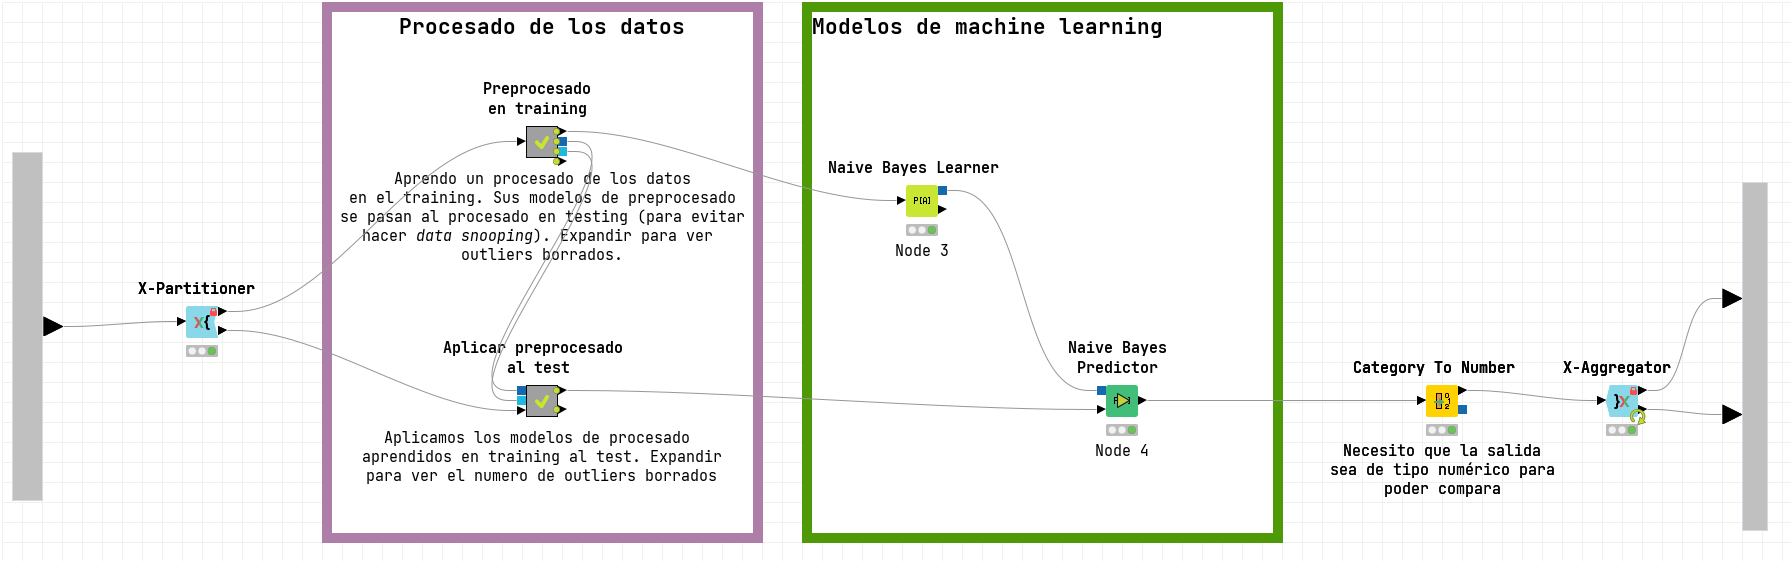
\includegraphics[width = 0.9 \textwidth]{dataset01_cv_naivebayes}
    \caption{Nodo de \emph{Cross Validation} para \emph{Naive Bayes}}
\end{figure}

Terminamos esta sección mostrando el proceso para Random Forest. De nuevo, no realizamos un preprocesado previo general para aplicar el algoritmo, como se muestra a continuación:

\begin{figure}[H]
    \centering
    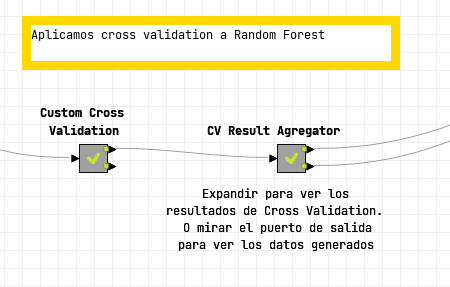
\includegraphics[width = 0.9 \textwidth]{dataset01_cv_pregeneral_randomforest}
    \caption{Preprocesado general previo a probar \emph{Random Forest}. En este caso tampoco estamos realizando ningún tipo de preprocesado previo a \emph{Custom Cross Validation}}
\end{figure}

Y de nuevo, nos encontramos con la misma situación dentro de \emph{Custom Cross Validation}. Simplemente pasamos a variable numérica la salida para que funcione bien el nodo de \lstinline{X-Aggregator}. Mostramos esto en la siguiente figura:

\begin{figure}[H]
    \centering
    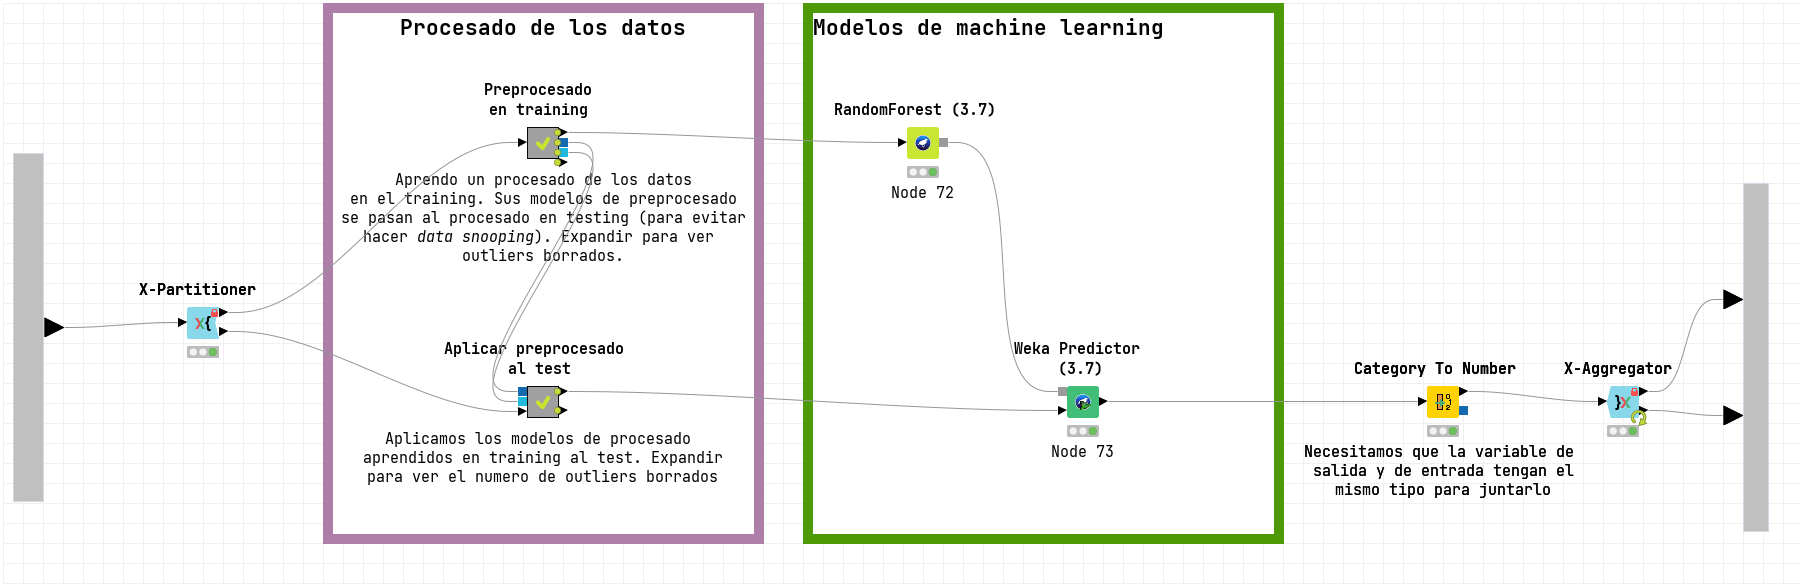
\includegraphics[width = 0.9 \textwidth]{dataset01_cv_randomforest}
    \caption{Nodo de \emph{Cross Validation} para \emph{Random Forest}}
\end{figure}

\pagebreak

\subsubsection{Mostrando los resultados obtenidos}

En primer lugar, mostramos la tabla que resume todos los resultados obtenidos tras el proceso de \emph{Cross Validation}:

\pagebreak

% Bibliografia
\bibliography{./References}
\bibliographystyle{ieeetr}

\end{document}
